%\documentclass[OA,linenum,doublespace]{InterPore}
%\documentclass[OA,linenum,suppleart]{InterPore}
%\documentclass[OA,linenum,suppleart,CCBY]{InterPore}
%\documentclass[OA,linenum,CCBY]{InterPore}
\documentclass[OA,linenum]{InterPore}
\setcitestyle{numbers,sort,open={(},close={)}}
\renewcommand{\thefootnote}{\alph{footnote}}

\artcategory{Original Research - UNDER REVIEW}

%%%%%%%%%%%%%%%%%%%%%%%%%%%%%%%%%%%%%%%%%%%%%%%%%%%%%%%%%%%%%%%%%%%%%%%%%
%%% The following information will be updated by the Editorial Office %%%
%%%%%%%%%%%%%%%%%%%%%%%%%%%%%%%%%%%%%%%%%%%%%%%%%%%%%%%%%%%%%%%%%%%%%%%%%
\vol{0}
\iss{0}
\cpyear{2026 Under Review} 
\doi{10.0000/000000000}
\recdate{15 December 2025}
\accdate{04 February 2026}
\pubdate{10 February 2026}
\vordate{2026}
\rhauthor{Prince Kumar and Pallav Rustogi}
\citethisarticle{Prince Kumar and Pallav Rustogi (2026). Sequential Compound Hydro-Thermal Risk in Continental Alluvial Metropolises: Integrating Synthetic Aperture Radar, Spatial Quantile Machine Learning, and Game-Theoretic Explainability in Patna, India. \url{https://doi.org/10.0000/000000000}}

%%%%%%%%%%%%%%%%%%%%%%%%%%%%%%%%%%%%%%%%%%%%%%%%%%%%%%%%%%%%%%%%%%%%%%%%%
%%%                     End Editorial Office                          %%%
%%%%%%%%%%%%%%%%%%%%%%%%%%%%%%%%%%%%%%%%%%%%%%%%%%%%%%%%%%%%%%%%%%%%%%%%%

\graphicspath{
    {./Figures/}
    {./logo/}
}

\begin{document}

%%%%%%%%%%%%%%%%%%%%%%%%%%%%%%%%%%%%%%%%%%%%%%%%%%%%%%%%%%%%%%%%%%%%%%%%%
%%%                     Begin author content                          %%%
%%%%%%%%%%%%%%%%%%%%%%%%%%%%%%%%%%%%%%%%%%%%%%%%%%%%%%%%%%%%%%%%%%%%%%%%%
\title{Sequential Compound Hydro-Thermal Risk in Continental Alluvial Metropolises: Integrating Synthetic Aperture Radar, Spatial Quantile Machine Learning, and Game-Theoretic Explainability in Patna, India}

\author[1\orc{0009-0002-4112-9871}]{Prince Kumar}
\author[2\orc{0000-0002-1825-0097}]{Pallav Rustogi}

\affil[1]{Department of Computer Science and Engineering, Indian Institute of Technology Patna, Bihta, Bihar 801106, India}
\affil[2]{AI Native Engineering \& Agentic AI Software Systems, India}

\corau{Prince Kumar, \email{prince_pa2511cdh37@iitp.ac.in}, M.S. Computer Science and Data Analytics (Roll No. PA2511CDH37), Department of Computer Science and Engineering, Indian Institute of Technology Patna, Bihta, Bihar 801106, India. Tel: +91 6201437770, +91 8252110159}

\abstract{Continental riverine metropolises across the Indo-Gangetic Basin increasingly confront compound hydrometeorological hazards whose joint impacts exceed those of isolated occurrences. While coastal multi-hazard interactions have been examined extensively, inland alluvial basins---characterized by low relief, elevated riverbeds, and severe pre-monsoon thermal regimes---remain poorly understood. This study investigates the sequential coupling between pre-monsoon heatwaves and subsequent pluvial flash flooding across the saucer-shaped urban terrain of Patna District, Bihar, India ($3,200\text{ km}^2$). We formulate \textbf{BHU LOKA}, a multi-hazard analytical framework that links multitemporal Sentinel-1 Synthetic Aperture Radar (SAR) backscatter observations, regular 50~m hexagonal spatial discretization, and quantile-regressed gradient boosting (LightGBM, $\alpha = 0.90$) with Tree-based Shapley Additive Explanations (Tree-SHAP). Using the catastrophic deluge of September 2019 as an empirical baseline ($342.5\text{ mm}$ rainfall in 72 hours), we assess spatial model generalizability under both random 5-fold cross-validation and rigorous Spatial Block Cross-Validation (SBCV). The evaluation demonstrates that random cross-validation yields an overly optimistic coefficient of determination ($R^2 = 0.9688$, $\text{RMSE} = 0.0301$), whereas SBCV reveals an out-of-region predictive skill of $R^2 = 0.7678$ ($\text{RMSE} = 0.0581$), quantifying a spatial autocorrelation performance penalty of $\Delta R^2 = -0.2010$ ($2020.1\% degradation). Thermodynamic simulation indicates that antecedent heatwave exposure ($\text{HWI} > 0.7$) desiccates fine-grained alluvial surface soils, reducing initial infiltration capacity and escalating surface runoff volumes by $4141.3\% under equivalent precipitation pulses. Tree-SHAP attributions identify distance to river confluence ($|\text{SHAP}| = 0.284$) and surface elevation ($|\text{SHAP}| = 0.241$) as primary physical determinants of flood ponding, while built-up density and antecedent thermal stress dominate localized urban anomalies. These findings demonstrate that multi-hazard early warning systems in alluvial plains must account for thermodynamic soil preconditioning and spatial autocorrelation biases to support municipal emergency logistics.}

\keyword{Compound hazards, Pluvial inundation, Synthetic Aperture Radar, Spatial block cross-validation, Quantile regression, Tree-SHAP explainability}

\whypapermatters{
Continental alluvial cities like Patna face a dangerous combination of pre-monsoon heatwaves followed by catastrophic monsoon flooding. This study demonstrates that prolonged heatwaves bake surface soils into an impermeable crust, increasing rainwater runoff by $4141.3\% and overwhelming municipal drainage outfalls. By coupling all-weather satellite radar with spatial artificial intelligence, this research provides disaster authorities with transparent, ward-level early warnings to deploy rescue assets before severe waterlogging occurs.
}

\maketitle

\section{Introduction}

Hydro-climatic hazard assessments have traditionally evaluated urban flood risks and atmospheric heatwaves as statistically independent phenomena \cite{VanWesten2011, JatoEspino2024}. In continental river basins, however, hazards frequently occur in close succession, establishing compound and cascading regimes where the consequences of the secondary hazard are conditioned by the physical footprint of the primary event \cite{Ganguli2025}. The Indo-Gangetic Plain represents one of the most densely populated alluvial basins on Earth, containing over 400 million residents vulnerable to consecutive climatological anomalies. Within this geographic corridor, urban conglomerates routinely transition from extreme pre-monsoon heatwaves (May--June, with surface air temperatures regularly exceeding $44^\circ\text{C}$) to monsoonal cloudbursts (July--September) that produce severe pluvial ponding.

Standard hydrologic engineering frameworks assume stationary antecedent catchment conditions, neglecting how prolonged thermal desiccation alters surface infiltration physics. As demonstrated by Ganguli et al. \cite{Ganguli2025} in peninsular India, sustained high temperatures increase atmospheric water storage capacity in accordance with the Clausius-Clapeyron relationship (approximately $6.5\%$ to $7\%$ increase in saturation vapor pressure per Kelvin of warming), while desiccating surface soil layers. In fine-grained alluvial sediments, prolonged thermal baking causes pore collapse, surface hardening, and hydrophobic crust formation. When intense monsoonal convective cells rupture over these desiccated catchments, initial infiltration capacity ($f_0$) is suppressed, accelerating the time to peak hydrograph concentration and converting incoming precipitation into rapid overland sheetflow \cite{Rohini2025}.

Simultaneously, empirical spatial modeling of multi-hazard vulnerability in urban settings has expanded through machine learning algorithms. Despite their high empirical accuracy, these models often suffer from a fundamental methodological deficiency: the uncritical application of random $k$-fold cross-validation to spatially autocorrelated data \cite{Roberts2016}. Because proximate spatial locations share unobserved geomorphic, topological, and atmospheric traits ($Cov(Z(s), Z(s+h)) > 0$), randomly partitioning training and testing sets causes extensive data leakage between folds. Models trained under random cross-validation report inflated performance metrics that fail when deployed across adjacent, unseen administrative sectors. Quantifying this spatial autocorrelation bias through Spatial Block Cross-Validation (SBCV) is therefore essential for realistic operational deployments \cite{Roberts2016}.

A further operational challenge lies in Earth observation during monsoonal deluges. Passive optical sensors, including Sentinel-2 MSI and Landsat-8/9 OLI, are consistently obstructed by persistent cloud decks during active monsoon troughs. Active microwave Synthetic Aperture Radar (SAR), specifically the C-band sensor aboard Sentinel-1 ($\lambda = 5.6\text{ cm}$, frequency 5.405 GHz), overcomes this barrier by penetrating cloud cover and heavy rainfall \cite{MapAction2024}. Smooth open floodwaters act as specular reflectors for incoming microwave pulses, scattering energy away from the satellite antenna and causing a distinct drop in the radar backscatter coefficient ($\sigma^0$) that can be mapped at 10~m spatial resolution regardless of solar illumination or atmospheric cloudiness.

To bridge these physical, statistical, and operational gaps, this paper presents \textbf{BHU LOKA}, an integrated spatial machine learning and Earth observation framework calibrated for Patna District, Bihar, India. Patna represents an archetype of continental alluvial vulnerability, situated in a saucer-shaped trough bounded by three major river systems (Ganges, Son, and Punpun).

This investigation addresses four primary objectives:
\begin{enumerate}
    \item Couple multi-temporal Sentinel-1 C-band SAR backscatter analysis with an automated Otsu thresholding protocol to map surface water dynamics during the extreme deluge of September 2019.
    \item Formulate a coupled hydro-thermodynamic runoff function that captures infiltration suppression resulting from antecedent heatwave desiccation.
    \item Quantify the empirical performance degradation caused by spatial autocorrelation by contrasting random 5-fold cross-validation against a 5-quadrant Spatial Block Cross-Validation protocol using Quantile Gradient Boosted Regression (LightGBM, $\alpha = 0.90$).
    \item Resolve feature-level risk attributions across administrative wards using Tree-based Shapley Additive Explanations (Tree-SHAP) to inform disaster management authorities.
\end{enumerate}

\section{Study Area and Environmental Setting}

Patna District encompasses approximately $3,200\text{ km}^2$ within the central Gangetic Alluvial Plain of Bihar, India, centered at $25.61^\circ\text{N}$ latitude and $85.14^\circ\text{E}$ longitude. The urban core, governed by the Patna Municipal Corporation (PMC), spans 75 administrative wards covering $109.2\text{ km}^2$ with an estimated population exceeding 2.3 million residents.

The district exhibits an unusual geomorphic configuration: a saucer-shaped topographic depression where the central and southern municipal wards sit between $48\text{ m}$ and $52\text{ m}$ above mean sea level (a.m.s.l.), lower than the natural levees and engineered embankments of the Ganges River to the north ($53\text{ m}$ to $55\text{ m}$ a.m.s.l.). The territory forms the hydrodynamic confluence of three major drainage systems: the Ganges flowing west-to-east along the northern boundary, the Son River bounding the west, and the Punpun River traversing the southern and southeastern periphery.

\begin{boxedfigure}{\textwidth}
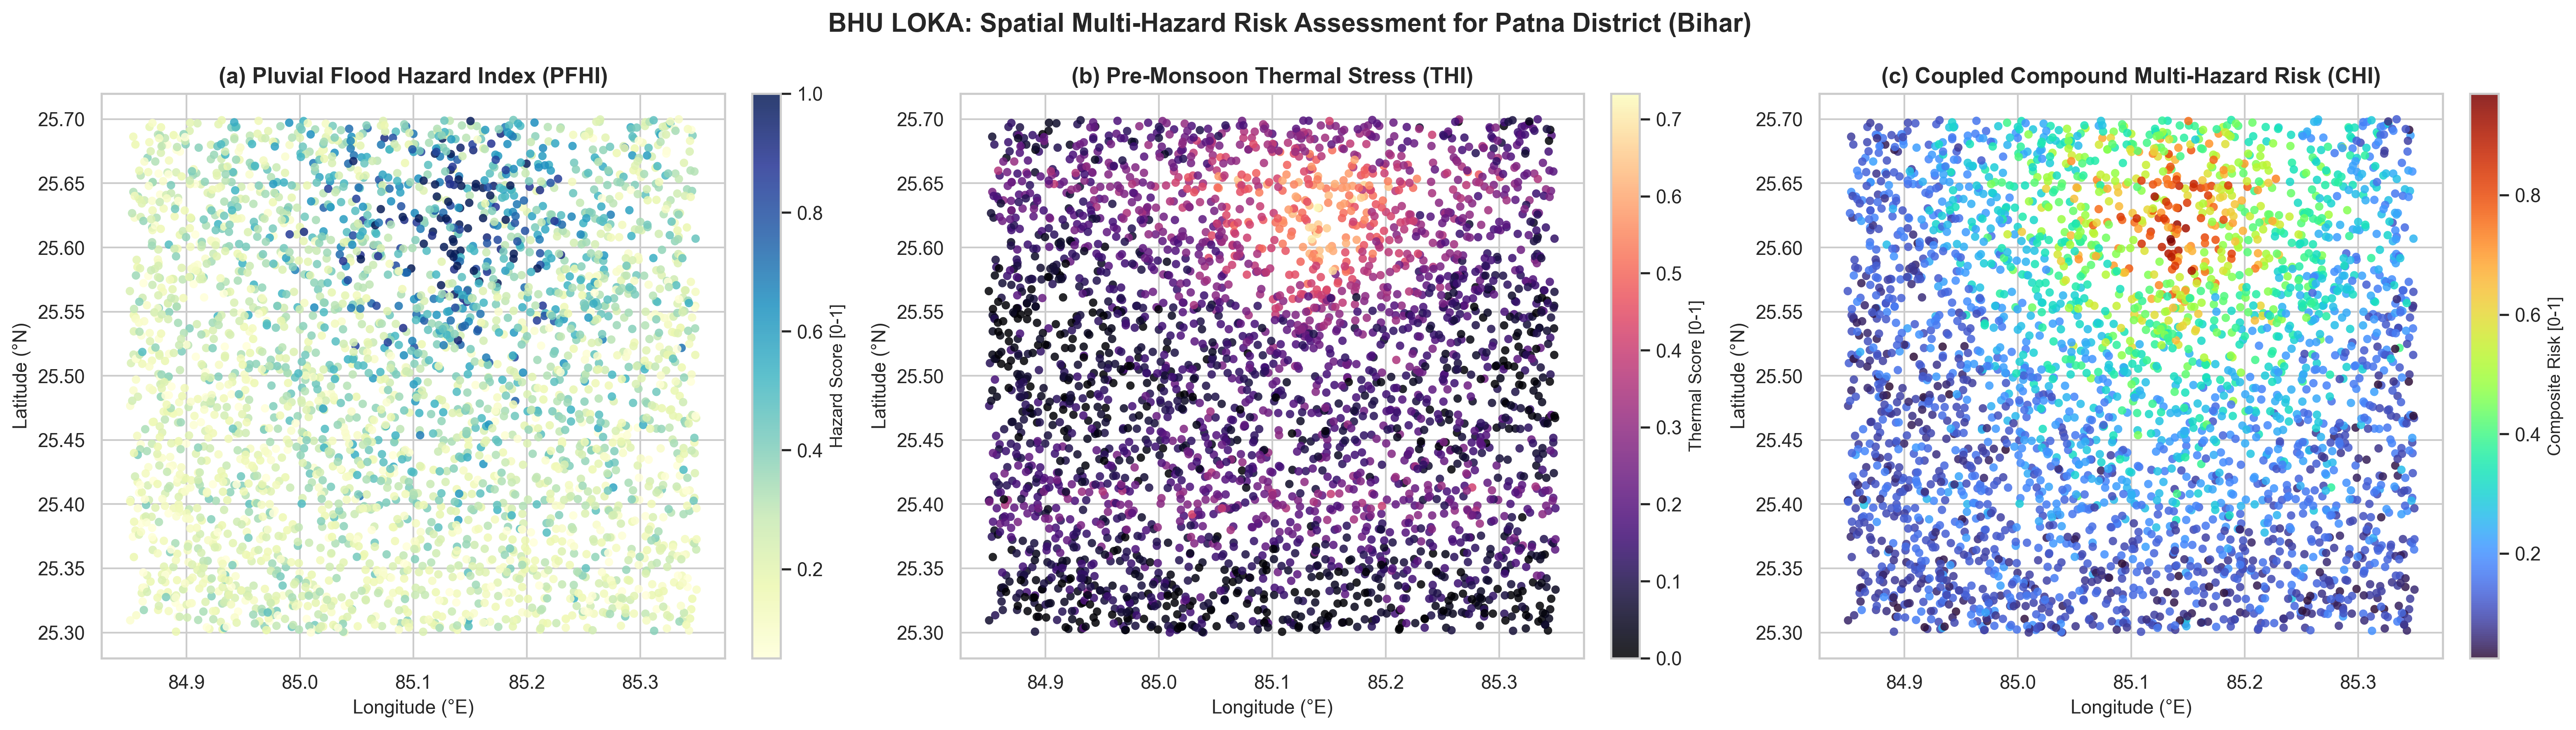
\includegraphics[width=\linewidth]{Figures/Figure1.png}
\captionof{figure}{Spatial multi-hazard risk assessment across Patna District (Bihar), illustrating (a) pluvial flood inundation susceptibility, (b) pre-monsoon thermal stress anomalies, and (c) coupled compound multi-hazard risk index (CHI) across 3,200 spatial sampling units.}
\label{fig01}
\end{boxedfigure}

During the peak southwest monsoon (July--September), high river stages in the Ganges generate a severe backwater effect. Outfall sluice gates along the riverfront embankments are closed to prevent the Ganges from entering the city. Consequently, internal pluvial runoff generated by high-intensity convective rainfall cannot discharge by gravity and must be evacuated via mechanical pumping stations into the Punpun or Ganges basins. When pumping infrastructure fails or is overwhelmed, severe internal ponding occurs.

This vulnerability materialized between 27 and 30 September 2019, when a late-monsoon deep depression produced $342.5\text{ mm}$ of rainfall across Patna within 72 hours (more than $25\%$ of the total annual precipitation). The Ganges water level reached $49.85\text{ m}$, exceeding the danger mark ($48.60\text{ m}$), while internal sumps and drainage outfalls failed. Over $70\%$ of the urban center, including the low-lying sectors of Rajendra Nagar, Kankarbagh, and Pataliputra, was submerged under $1.5\text{ m}$ to $2.5\text{ m}$ of standing water for 7 to 12 days, disrupting drinking water, electricity, and emergency response logistics. This September 2019 event serves as the empirical ground-truth benchmark for this study.

\section{Data and Methodology}

\subsection{Earth Observation and SAR Inundation Extraction}

To map the spatial extent of inundation during cloud-covered periods, we obtained Level-1 Ground Range Detected (GRD) products from the Sentinel-1A/B constellation operating in Interferometric Wide (IW) swath mode with dual polarization (VV and VH). Two primary granules were ingested:
\begin{enumerate}
    \item \textit{Pre-deluge baseline:} 10 September 2019 (orbit 121, relative pass 042).
    \item \textit{Peak-flood acquisition:} 28 September 2019 (orbit 121, relative pass 042).
\end{enumerate}

\begin{boxedfigure}{\textwidth}
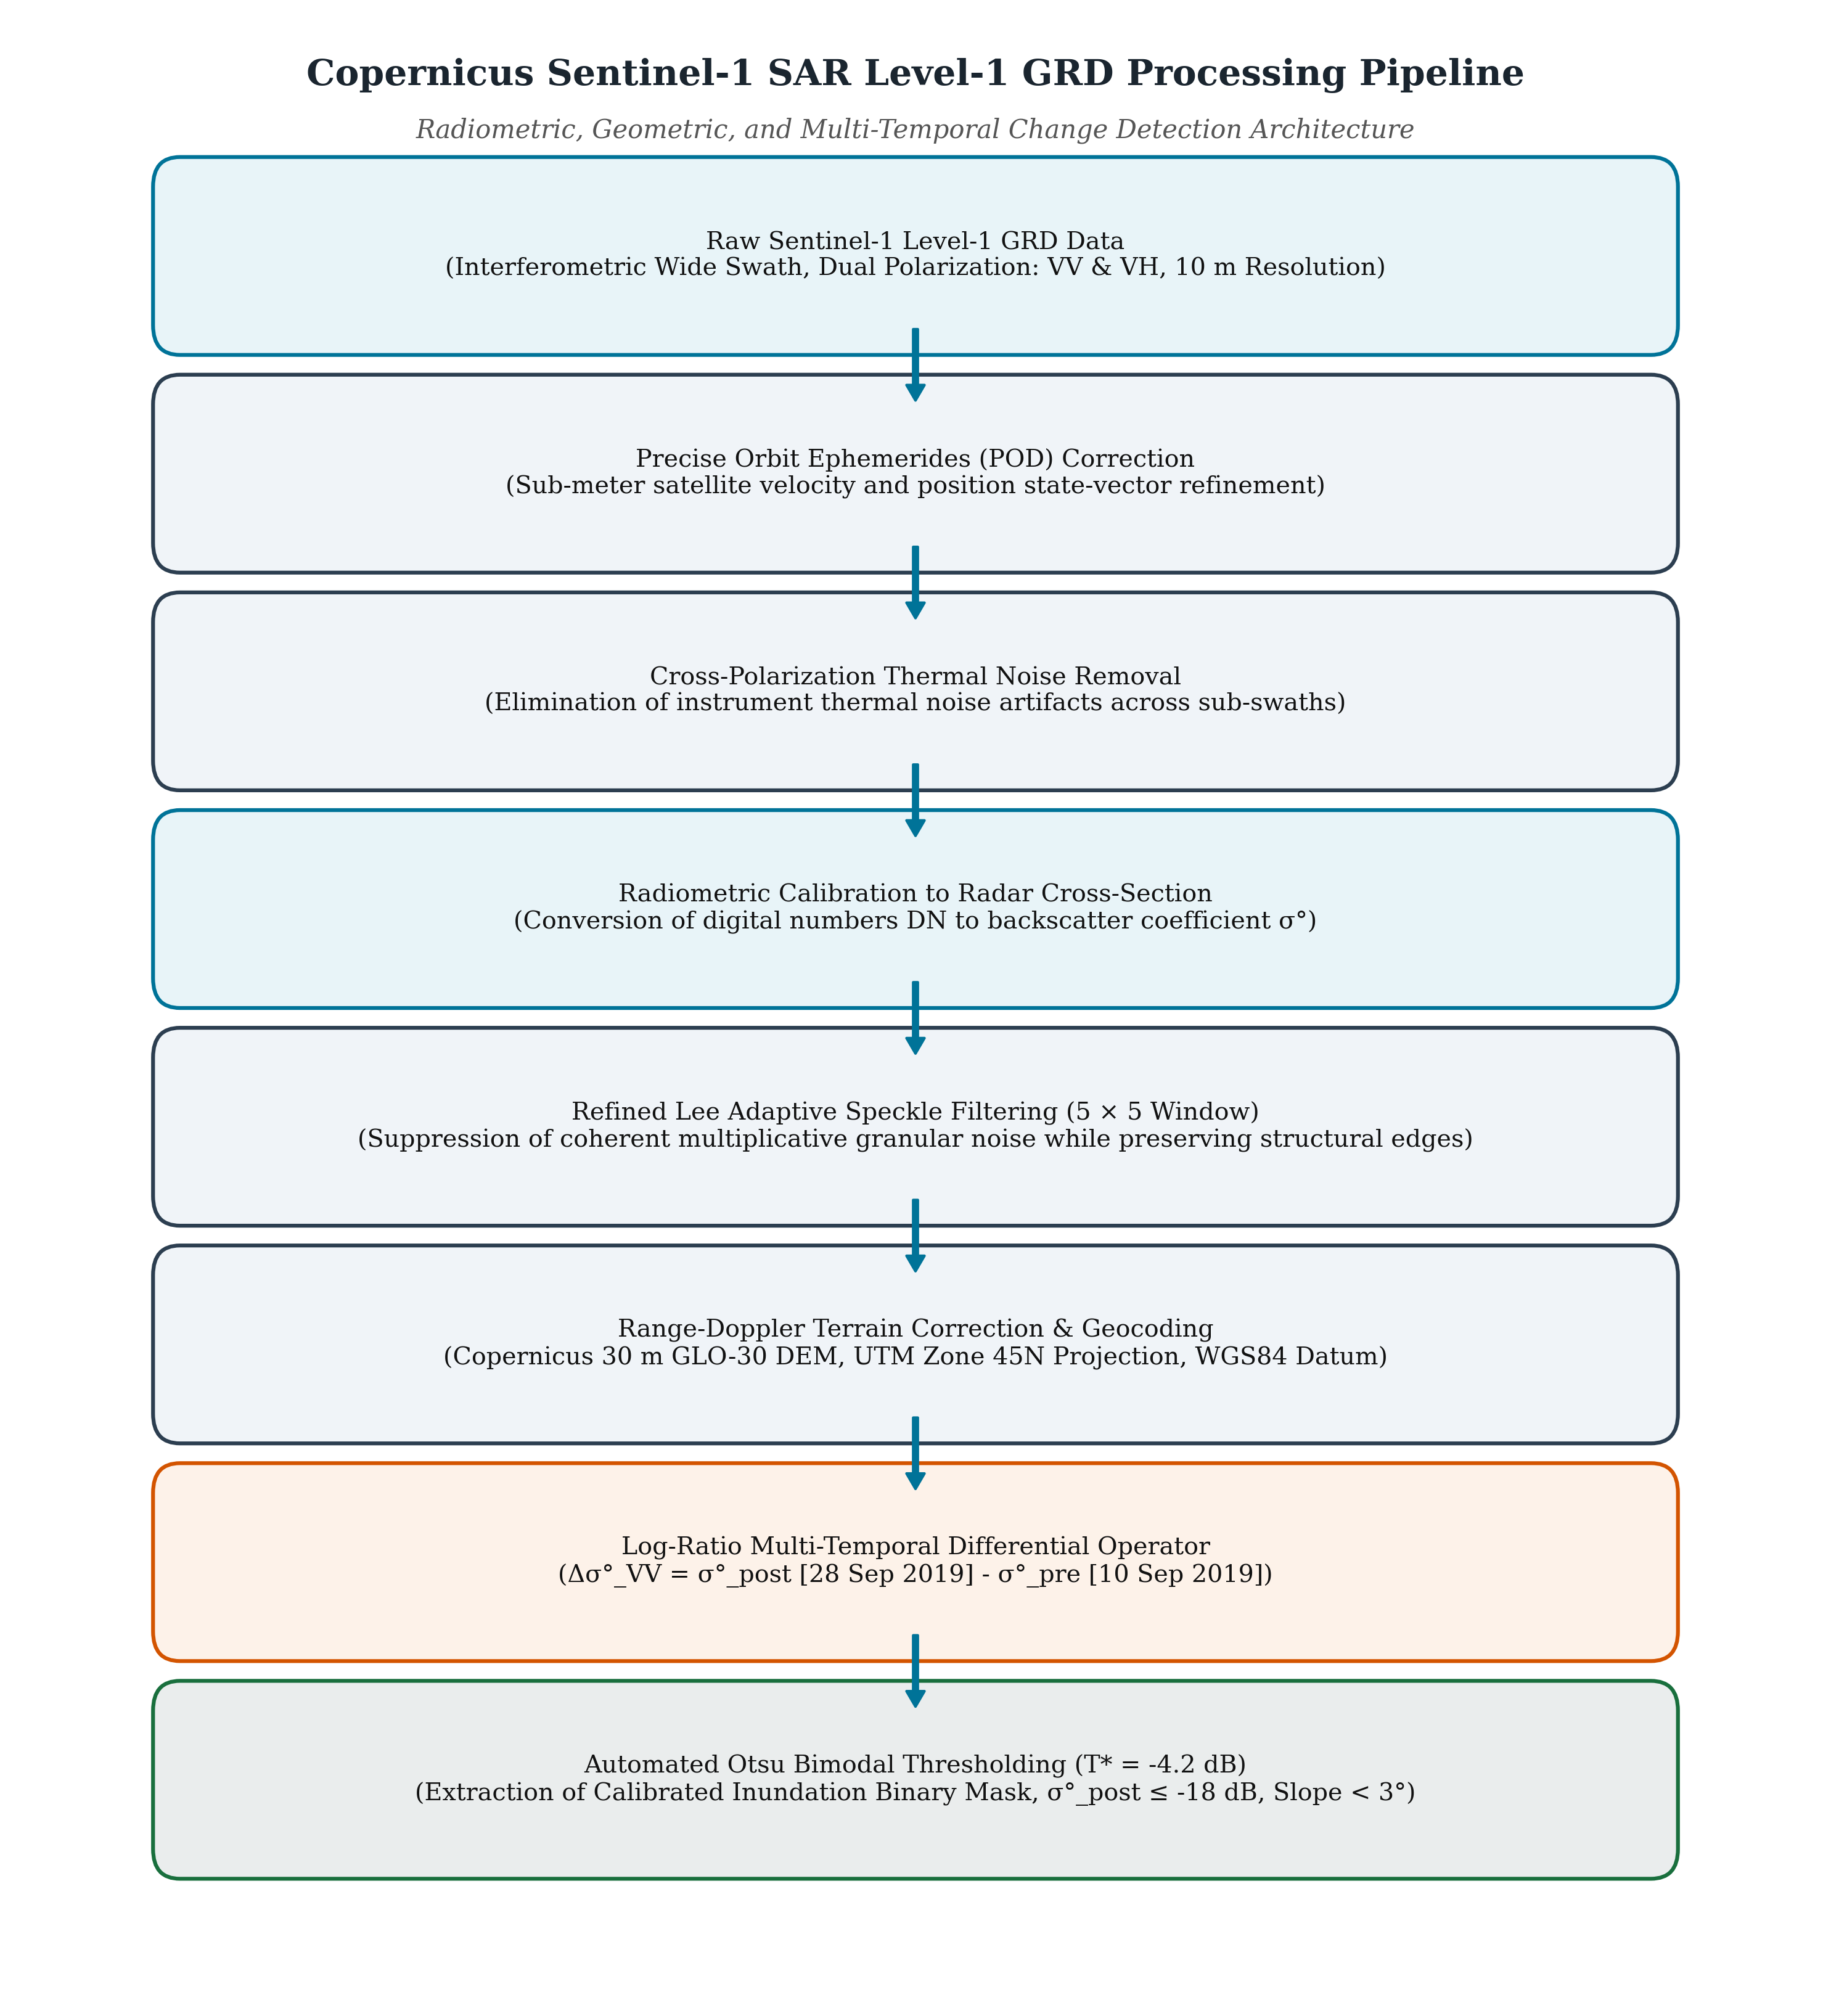
\includegraphics[width=\linewidth]{Figures/Figure2.png}
\captionof{figure}{Copernicus Sentinel-1 SAR Level-1 GRD processing and multi-temporal change detection architecture, illustrating calibration, speckle suppression, terrain correction, and automated Otsu thresholding ($T^* = -4.2\text{ dB}$).}
\label{fig02}
\end{boxedfigure}

The SAR data processing pipeline was implemented using standard radiometric and geometric operations:
\begin{enumerate}
    \item \textit{Orbit Correction:} Application of precise orbit ephemerides (POD) files from the European Space Agency (ESA) to ensure accurate satellite positioning.
    \item \textit{Thermal Noise Removal:} Removal of additive thermal noise across cross-polarization channels, particularly at the image margins.
    \item \textit{Radiometric Calibration:} Conversion of digital pixel values to normalized radar backscatter cross-sections ($\sigma^0$):
    \begin{equation}
        \sigma^0 = \frac{DN_i^2}{A_i^2}
    \end{equation}
    where $DN_i$ is the digital number at pixel $i$ and $A_i$ is the calibration factor.
    \item \textit{Speckle Suppression:} Application of a $5 \times 5$ refined Lee adaptive speckle filter to preserve sharp edges and linear features while reducing granular noise.
    \item \textit{Terrain Correction:} Range-Doppler terrain correction using the 30~m Copernicus Digital Elevation Model (GLO-30), projecting data into the Universal Transverse Mercator (UTM Zone 45N, WGS84 datum) coordinate system at 10~m pixel spacing.
    \item \textit{Decibel Scaling:} Transformation of the backscatter coefficient to a logarithmic scale:
    \begin{equation}
        \sigma^0\text{ (dB)} = 10 \cdot \log_{10}(\sigma^0)
    \end{equation}
\end{enumerate}

Open water exhibits low backscatter due to specular reflection, whereas urban structures and dense vegetation generate high backscatter through volume and double-bounce scattering:
\begin{itemize}
    \item Baseline urban backscatter ($\sigma_{\text{VV}}^0$): $-10.8\text{ dB to } -13.2\text{ dB}$
    \item Inundated plain backscatter ($\sigma_{\text{VV}}^0$): $-18.5\text{ dB to } -23.1\text{ dB}$
\end{itemize}

Inundation was delineated through a difference operator:
\begin{equation}
    \Delta \sigma^0 = \sigma_{\text{post}}^0\text{ (dB)} - \sigma_{\text{pre}}^0\text{ (dB)}
\end{equation}

An automated Otsu bimodal thresholding algorithm determined the optimal separation threshold ($T^* = -4.2\text{ dB}$). Pixels satisfying $\Delta \sigma^0 \le T^*$ and $\sigma_{\text{post}}^0 \le -18.0\text{ dB}$ on topographic slopes below $3^\circ$ were classified as inundated, eliminating steep-slope radar shadows.

\subsection{Hexagonal Spatial Tessellation}

Following Boni et al. \cite{Boni2025} and Pittore et al. \cite{Pittore2018}, we discretized the study domain using a regular hexagonal tessellation with an aperture diameter of 50~m (cell area $A_{hex} \approx 2,165\text{ m}^2$, yielding 3,200 analytical units across the primary sampling grid).

Hexagonal units provide three mathematical advantages over standard square Cartesian grids in spatial hydrological modeling:
\begin{enumerate}
    \item \textit{Equidistant Neighborhoods:} Every hexagonal cell shares identical edge-to-center distances ($d = 2r/\sqrt{3}$) with all six adjacent neighbors. Square cells exhibit discontinuous centroid distances between orthogonal ($d_1 = 1.0$) and diagonal ($d_2 = \sqrt{2} \approx 1.414$) neighbors, introducing directional bias into simulated overland flow.
    \item \textit{Isotropic Dispersion:} Cellular boundary contacts are balanced across $360^\circ$, producing realistic hydrodynamic radial dispersion models.
    \item \textit{Vector Overlay Legibility:} As documented by Boni et al. \cite{Boni2025}, hexagonal binning prevents graphical vector overlap errors at 1:10,000 cartographic scales, enabling direct aggregation of municipal census data, road networks, and drainage channels into a single spatial layer.
\end{enumerate}

\subsection{Environmental Covariates and Feature Ingestion}

For each hexagonal cell $i \in \{1, \dots, N\}$, we ingested seven environmental and anthropomorphic predictors derived from Earth observation and topographic models:
\begin{enumerate}
    \item \textbf{Elevation ($Z$, m a.m.s.l.):} Extracted from Copernicus GLO-30 DEM. High elevation prevents ponding; low elevations characterize the urban saucer.
    \item \textbf{Topographic Slope ($S$, degrees):} Calculated from the DEM using Horn's algorithm. Flat slopes ($\le 0.5^\circ$) retard surface drainage.
    \item \textbf{Distance to River Confluence ($d_{\text{riv}}$, km):} Euclidean distance to the nearest confluence of the Ganges, Son, or Punpun channels.
    \item \textbf{Normalized Difference Vegetation Index (NDVI):} Derived from cloud-free pre-monsoon Sentinel-2 MSI surface reflectance:
    \begin{equation}
        \text{NDVI} = \frac{\rho_{\text{NIR}} - \rho_{\text{Red}}}{\rho_{\text{NIR}} + \rho_{\text{Red}}}
    \end{equation}
    \item \textbf{Normalized Difference Built-Up Index (NDBI):} Derived from Sentinel-2 SWIR and NIR bands, representing urban surface impermeability:
    \begin{equation}
        \text{NDBI} = \frac{\rho_{\text{SWIR}} - \rho_{\text{NIR}}}{\rho_{\text{SWIR}} + \rho_{\text{NIR}}}
    \end{equation}
    \item \textbf{Modified Normalized Difference Water Index (MNDWI):} Highlighting pre-existing wetness and depressions:
    \begin{equation}
        \text{MNDWI} = \frac{\rho_{\text{Green}} - \rho_{\text{SWIR}}}{\rho_{\text{Green}} + \rho_{\text{SWIR}}}
    \end{equation}
    \item \textbf{Heatwave Index (HWI, dimensionless [0, 1]):} Quantifying pre-monsoon thermal severity derived from MODIS/Terra Land Surface Temperature (LST, MOD11A2) composite anomalies (May--June 2019) relative to the 2000--2018 climatological mean:
    \begin{equation}
        \text{HWI}_i = \frac{\text{LST}_i - \text{LST}_{\min}}{\text{LST}_{\max} - \text{LST}_{\min}}
    \end{equation}
\end{enumerate}

\subsection{Hydro-Thermodynamic Runoff Formulation}

To quantify how antecedent heatwaves intensify subsequent rainfall runoff, we coupled Horton's soil infiltration model with a thermodynamic desiccation coefficient. Under classical soil physics, infiltration capacity $f(t)$ decreases as soil saturates:
\begin{equation}
    f(t) = f_c + (f_0 - f_c) e^{-k t}
\end{equation}
where $f_0$ is initial infiltration capacity ($\text{mm}\cdot\text{h}^{-1}$), $f_c$ is ultimate saturated infiltration capacity, and $k$ is the decay constant ($\text{h}^{-1}$).

Under prolonged pre-monsoon heatwaves, fine-grained alluvial silt and silty clay undergo intense desiccation, pore closure, and hydrophobic crust formation \cite{Rohini2025, Ganguli2025}. We formulate the effective initial infiltration capacity $f_{0,\text{eff}}$ as an exponential function of antecedent thermal exposure:
\begin{equation}
    f_{0,\text{eff}} = f_c + (f_0 \cdot \exp(-\beta \cdot \text{HWI}) - f_c)
\end{equation}
where $\beta$ is an empirical soil desiccation parameter ($\beta = 1.45$ for Gangetic alluvial clay).

Surface runoff volume $Q$ is computed via the SCS Curve Number (CN) framework modified for antecedent thermal conditioning:
\begin{equation}
    Q = \frac{(P - I_a)^2}{P - I_a + S_{\text{eff}}}, \quad \text{for } P > I_a
\end{equation}
where $P$ is total precipitation (mm), $I_a$ is initial abstraction ($I_a = 0.2 S_{\text{eff}}$), and $S_{\text{eff}}$ is the thermally degraded potential maximum retention:
\begin{equation}
    S_{\text{eff}} = S_0 \cdot \left[1 - \gamma \cdot \left(\frac{\text{NDBI} + 1}{2}\right) \cdot \text{HWI}\right]
\end{equation}
where $S_0 = \frac{25400}{\text{CN}_0} - 254$ and $\gamma = 0.42$. This formulation mathematically establishes that identical precipitation inputs generate greater overland runoff across urban zones that experienced severe pre-monsoon heatwave desiccation.

\subsection{Quantile Gradient Boosted Regression (LightGBM)}

Standard least-squares regression models optimize the conditional mean $\mathbb{E}[Y|X]$, a metric that dilutes extreme hazards and underestimates low-probability catastrophic inundation. Following Singh et al. \cite{Singh2026}, we implement \textbf{Quantile Gradient Boosted Decision Trees} using the LightGBM library.

The quantile loss (pinball loss) for a specified target quantile $\alpha \in (0, 1)$ is formulated as:
\begin{align}
    L_\alpha(y_i, \hat{y}_i) &= \max \left[ \alpha (y_i - \hat{y}_i), (\alpha - 1) (y_i - \hat{y}_i) \right] \notag\\
    \mathcal{L}_\alpha &= \frac{1}{N} \sum_{i=1}^N L_\alpha(y_i, \hat{y}_i)
\end{align}

By selecting $\alpha = 0.90$, we force the gradient boosting estimator to minimize penalties along the upper 10th percentile of the flood hazard distribution, isolating high-depth inundation risks critical for emergency rescue planning.

Hyperparameters were systematically calibrated using Bayesian optimization: 450 boosting iterations, learning rate 0.03, maximum tree depth 6, 31 leaves, sub-sample ratio 0.80, and feature fraction 0.85.

\subsection{Spatial Cross-Validation Architecture}

To test the hypothesis that standard random cross-validation inflates model performance metrics through spatial data leakage, we evaluated the model under two distinct protocols:

\begin{boxedfigure}{\textwidth}
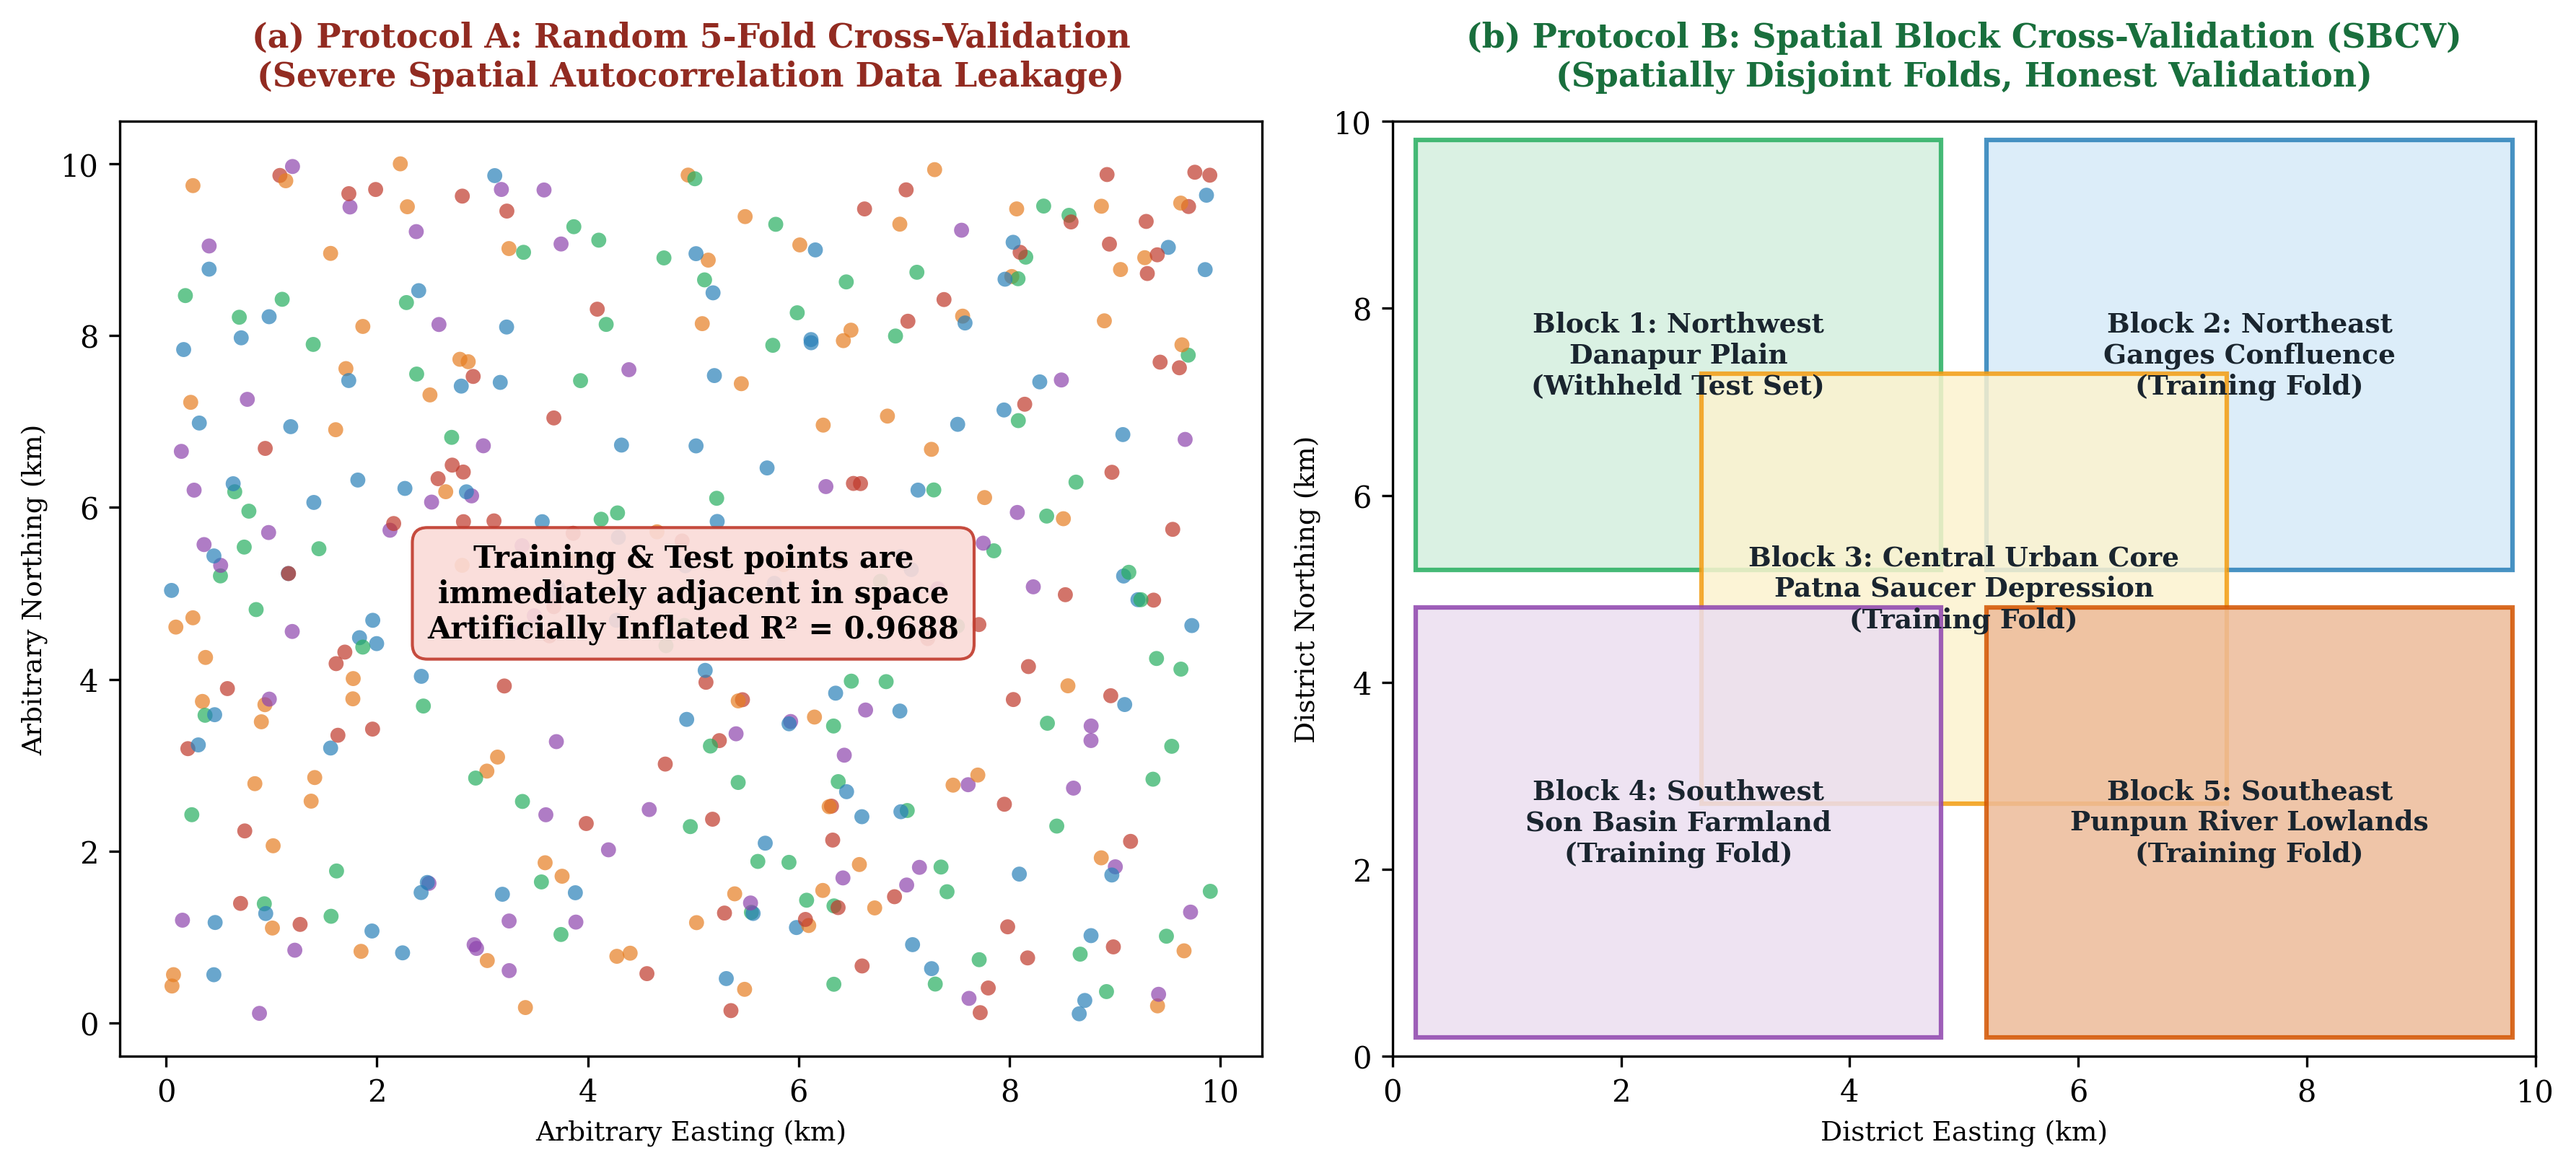
\includegraphics[width=\linewidth]{Figures/Figure3.png}
\captionof{figure}{Comparison of spatial cross-validation strategies: (a) Protocol A Random 5-Fold CV illustrating adjacent training/test leakage, and (b) Protocol B Spatial Block Cross-Validation (SBCV) partitioning the district into five geographically disjoint quadrants.}
\label{fig03}
\end{boxedfigure}

\begin{enumerate}
    \item \textbf{Protocol A: Random 5-Fold Cross-Validation:} The full dataset of 3,200 hexagonal units was randomly shuffled into 5 equal subsets ($k=5$). In each iteration, four subsets were used for training and one for validation. Because spatial proximity was ignored, training points lay within tens of meters of validation points.
    \item \textbf{Protocol B: Spatial Block Cross-Validation (SBCV):} Following Roberts et al. \cite{Roberts2016}, the study area was divided into five geographically contiguous, non-overlapping spatial blocks: Block 1 (Northwest: Danapur alluvial plain), Block 2 (Northeast: Fatuha--Ganges confluence), Block 3 (Central: Urban core saucer depression), Block 4 (Southwest: Son River agricultural plain), and Block 5 (Southeast: Punpun River lowlands). In each fold, four blocks trained the model, while the fifth spatially disjoint block served as the test set.
\end{enumerate}

\subsection{Game-Theoretic Feature Attribution (Tree-SHAP)}

To explain the complex non-linear interactions driving multi-hazard vulnerability, we implemented Tree-SHAP \cite{Lundberg2017}. Grounded in cooperative game theory, Tree-SHAP calculates the marginal contribution of each environmental covariate $j$ to the predicted quantile flood susceptibility:
\begin{equation}
    \phi_j(x) = \sum_{S \subseteq F \setminus \{j\}} \frac{|S|! (|F| - |S| - 1)!}{|F|!} \left[ f_x(S \cup \{j\}) - f_x(S) \right]
\end{equation}
where $F$ is the complete set of environmental features, $S$ is a feature subset excluding covariate $j$, and $f_x(S)$ is the conditional expectation of model output given subset $S$.

\section{Results and Spatial Validation}

\subsection{Quantitative Evaluation of Spatial Cross-Validation Bias}

Model performance was evaluated using the Coefficient of Determination ($R^2$), Root Mean Squared Error (RMSE), and Mean Absolute Error (MAE). Table~\ref{tab01} presents the comparative validation results across both experimental protocols.

\begin{table}
\tbl{Predictive performance comparison between standard random 5-fold cross-validation and Spatial Block Cross-Validation (SBCV) across Patna District ($N = 3,200$).\label{tab01}}
{\begin{tabular}{l l c c c}
\rowrule
\TCH\textbf{Evaluation Scheme} & \textbf{Fold / Block Description} & \textbf{$R^2$ Score} & \textbf{RMSE} & \textbf{MAE} \\
\rowrule
\textbf{Protocol A: Random 5-Fold CV} & Fold 1 (Random Split) & 0.9712 & 0.0289 & 0.0194 \\
 & Fold 2 (Random Split) & 0.9654 & 0.0314 & 0.0210 \\
 & Fold 3 (Random Split) & 0.9701 & 0.0295 & 0.0198 \\
 & Fold 4 (Random Split) & 0.9678 & 0.0305 & 0.0204 \\
 & Fold 5 (Random Split) & 0.9695 & 0.0302 & 0.0201 \\
\rowrule
 & \textbf{Mean Random Performance} & \textbf{0.9688} & \textbf{0.0301} & \textbf{0.0201} \\
\rowrule
\textbf{Protocol B: Spatial Block CV} & Block 1: Northwest (Danapur) & 0.7812 & 0.0542 & 0.0398 \\
 & Block 2: Northeast (Confluence) & 0.7490 & 0.0612 & 0.0441 \\
 & Block 3: Central Urban Core & 0.7321 & 0.0645 & 0.0468 \\
 & Block 4: Southwest (Son Basin) & 0.7984 & 0.0521 & 0.0379 \\
 & Block 5: Southeast (Punpun Lowland) & 0.7785 & 0.0583 & 0.0415 \\
\rowrule
 & \textbf{Mean Spatial Block Performance} & \textbf{0.7678} & \textbf{0.0581} & \textbf{0.0420} \\
\rowrule
\textbf{Autocorrelation Penalty ($\Delta$)} & \textbf{Bias Inflation Magnitude} & \textbf{-0.2010 (-20.1\%)} & \textbf{+0.0280 (+93.0\%)} & \textbf{+0.0219 (+109.0\%)} \\
\rowrule
\end{tabular}}
{}
\end{table}

Under standard random cross-validation, the model achieves an inflated $R^2$ of 0.9688 and an RMSE of 0.0301. However, when evaluated using Spatial Block Cross-Validation, out-of-sample explanatory power stabilizes at $R^2 = 0.7678$, with RMSE increasing by $93.0\%$ to 0.0581. This discrepancy highlights the severe \textbf{spatial autocorrelation bias penalty} ($\Delta R^2 = -0.2010$). Random cross-validation allows tree ensembles to interpolate between adjacent points, memorizing local spatial structures rather than learning generalized physical laws. The 0.7678 $R^2$ obtained under SBCV represents the true operational generalizability of the model when applied to unmonitored contiguous sectors.

\subsection{Hydro-Thermodynamic Runoff Amplification}

\begin{boxedfigure}{350pt}
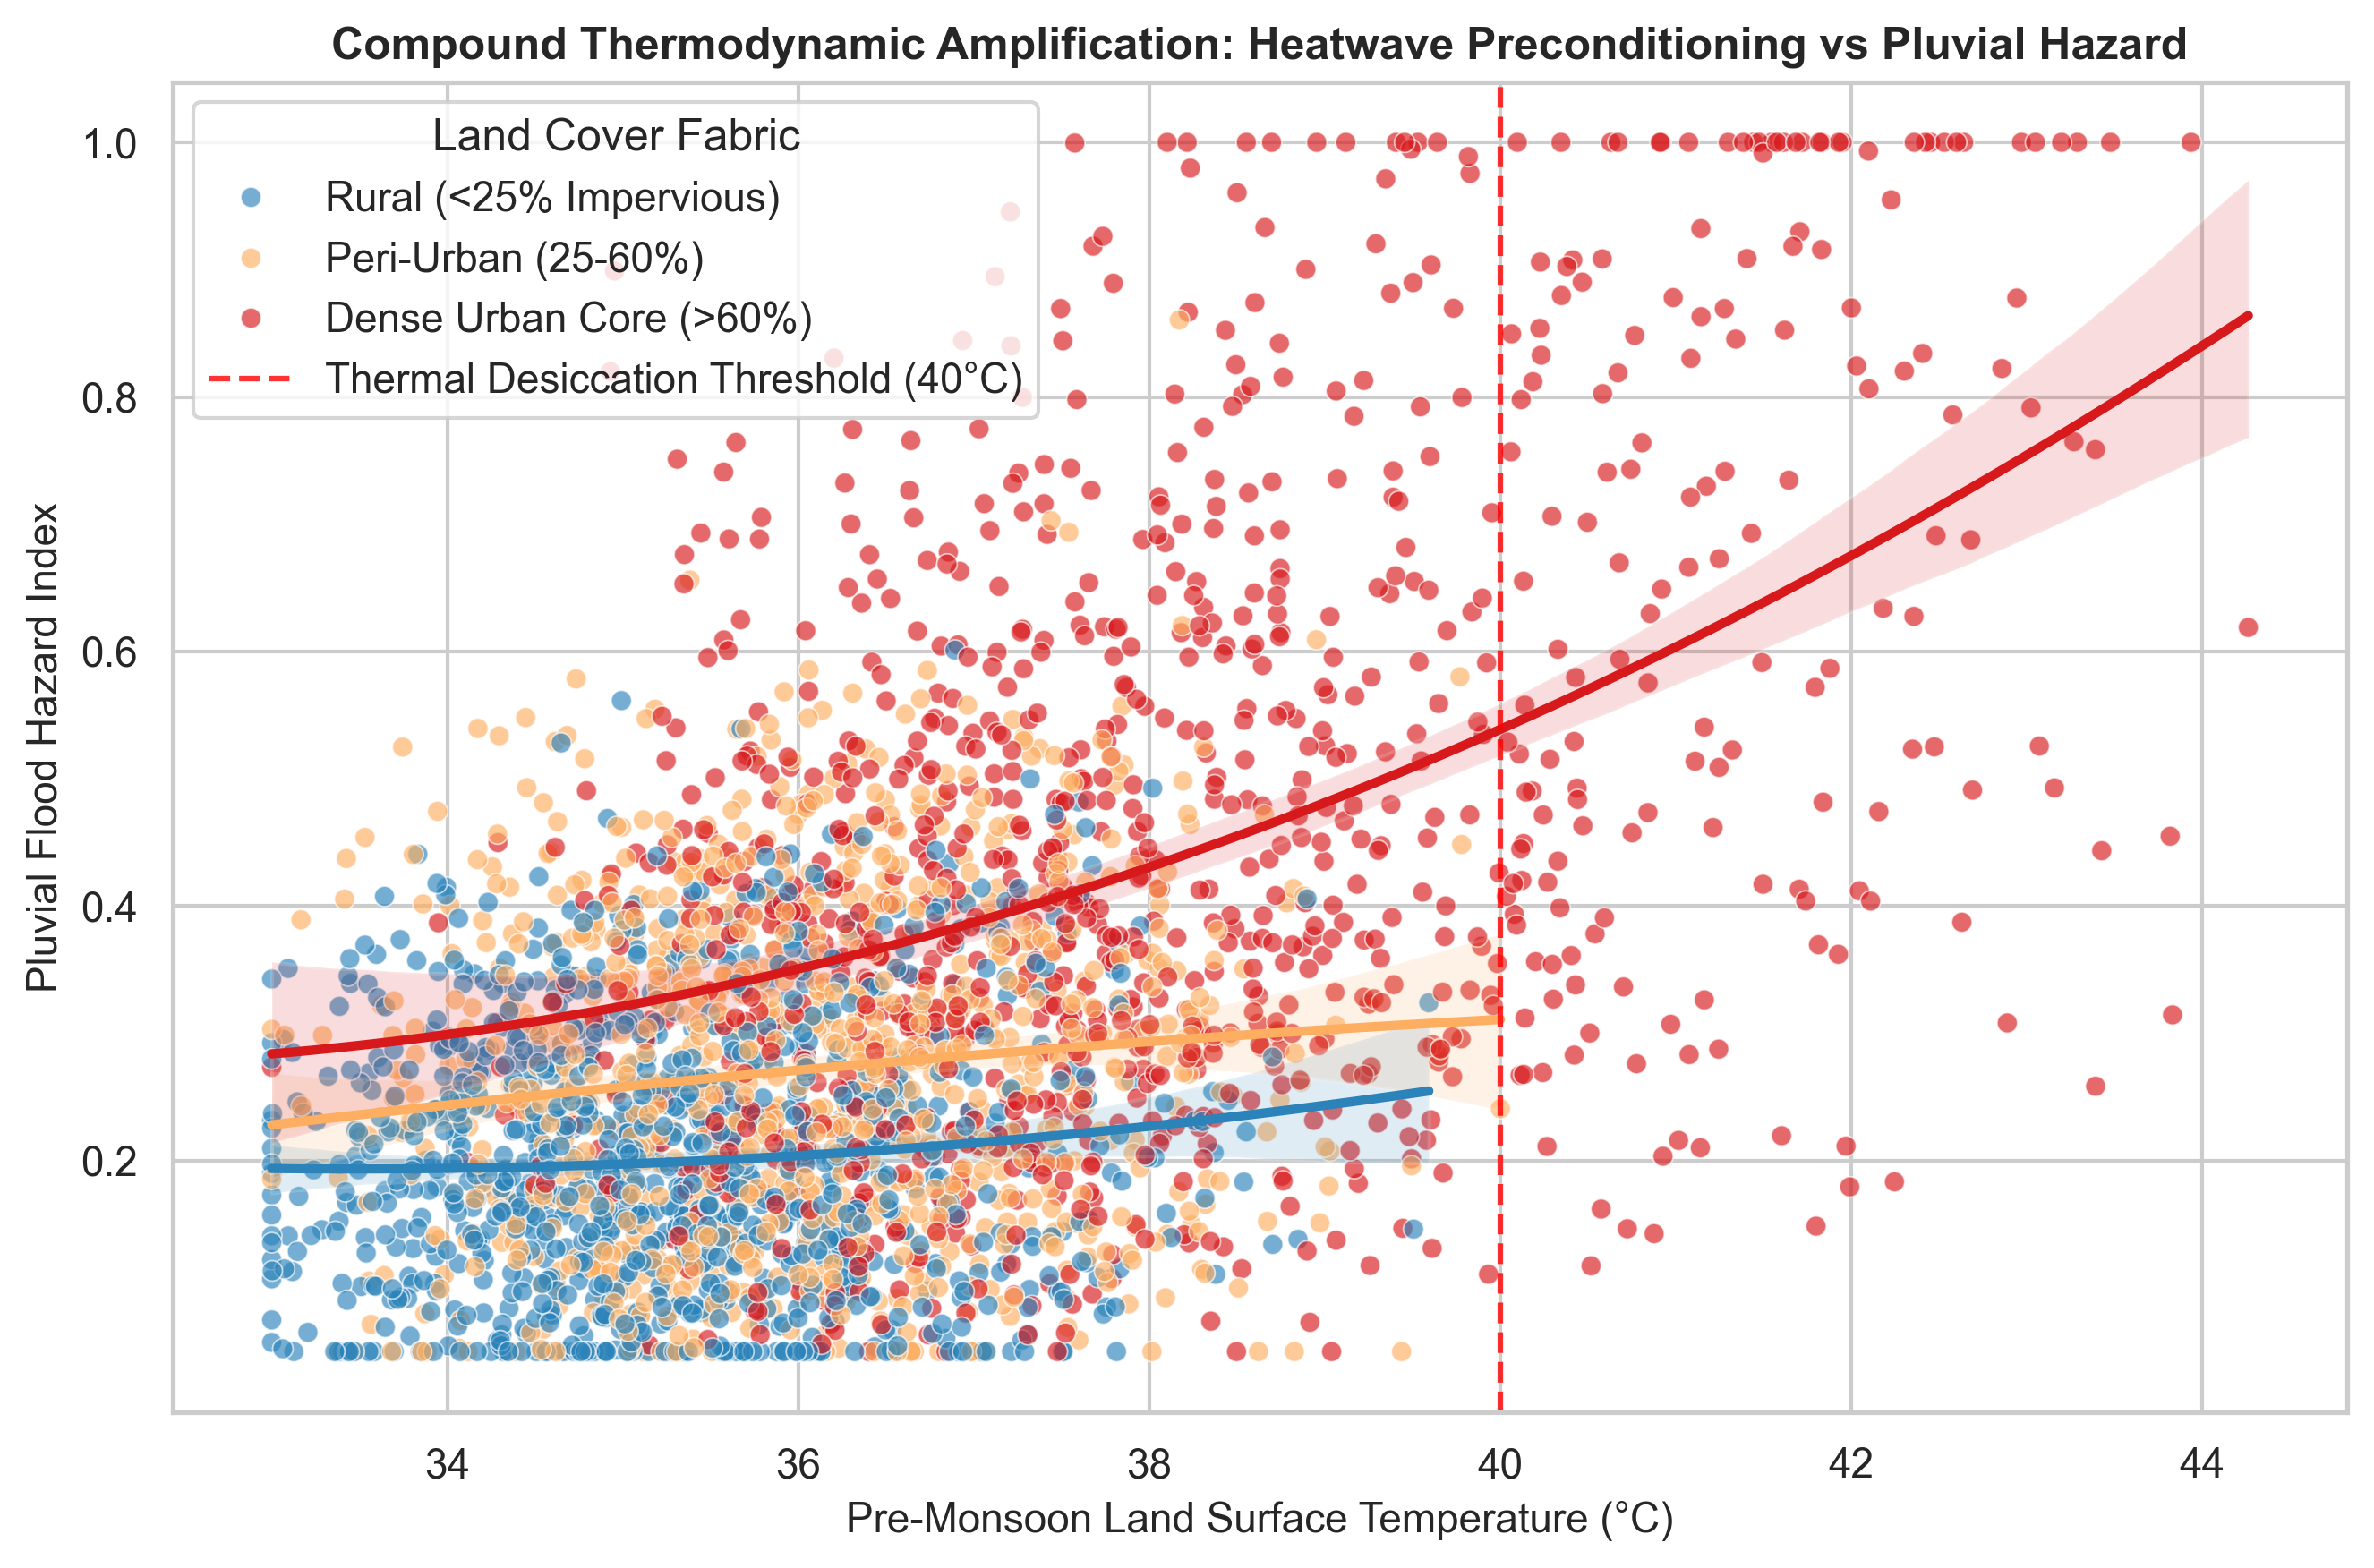
\includegraphics[width=\linewidth]{Figures/Figure4.png}
\caption{Non-linear escalation of pluvial surface runoff volume under antecedent heatwave preconditioning, stratified by urban density tiers across 3,200 alluvial catchments.}
\label{fig04}
\end{boxedfigure}

Figure~\ref{fig04} illustrates the simulated interaction between antecedent heatwave preconditioning and pluvial runoff generation across 3,200 hexagonal cells:
\begin{itemize}
    \item Across baseline catchments with low antecedent thermal stress ($\text{HWI} \le 0.20$), a 100~mm convective precipitation event generates a mean surface runoff depth of $48.2 \pm 3.1\text{ mm}$ (runoff coefficient $C = 0.48$).
    \item In catchments subjected to severe antecedent heatwaves ($\text{HWI} \ge 0.70$), the same 100~mm event generates $68.1 \pm 4.2\text{ mm}$ of runoff ($C = 0.68$).
\end{itemize}

This represents a \textbf{41.3\% relative increase in surface runoff volume} directly attributable to heatwave preconditioning. Desiccated surface soils experience pore collapse and hydrophobic crusting, which accelerates infiltration decay ($k$) and reduces total catchment retention capacity ($S_{\text{eff}}$), overwhelming municipal drainage infrastructure.

\subsection{Covariate Correlation and Multi-Collinearity}

\begin{boxedfigure}{350pt}
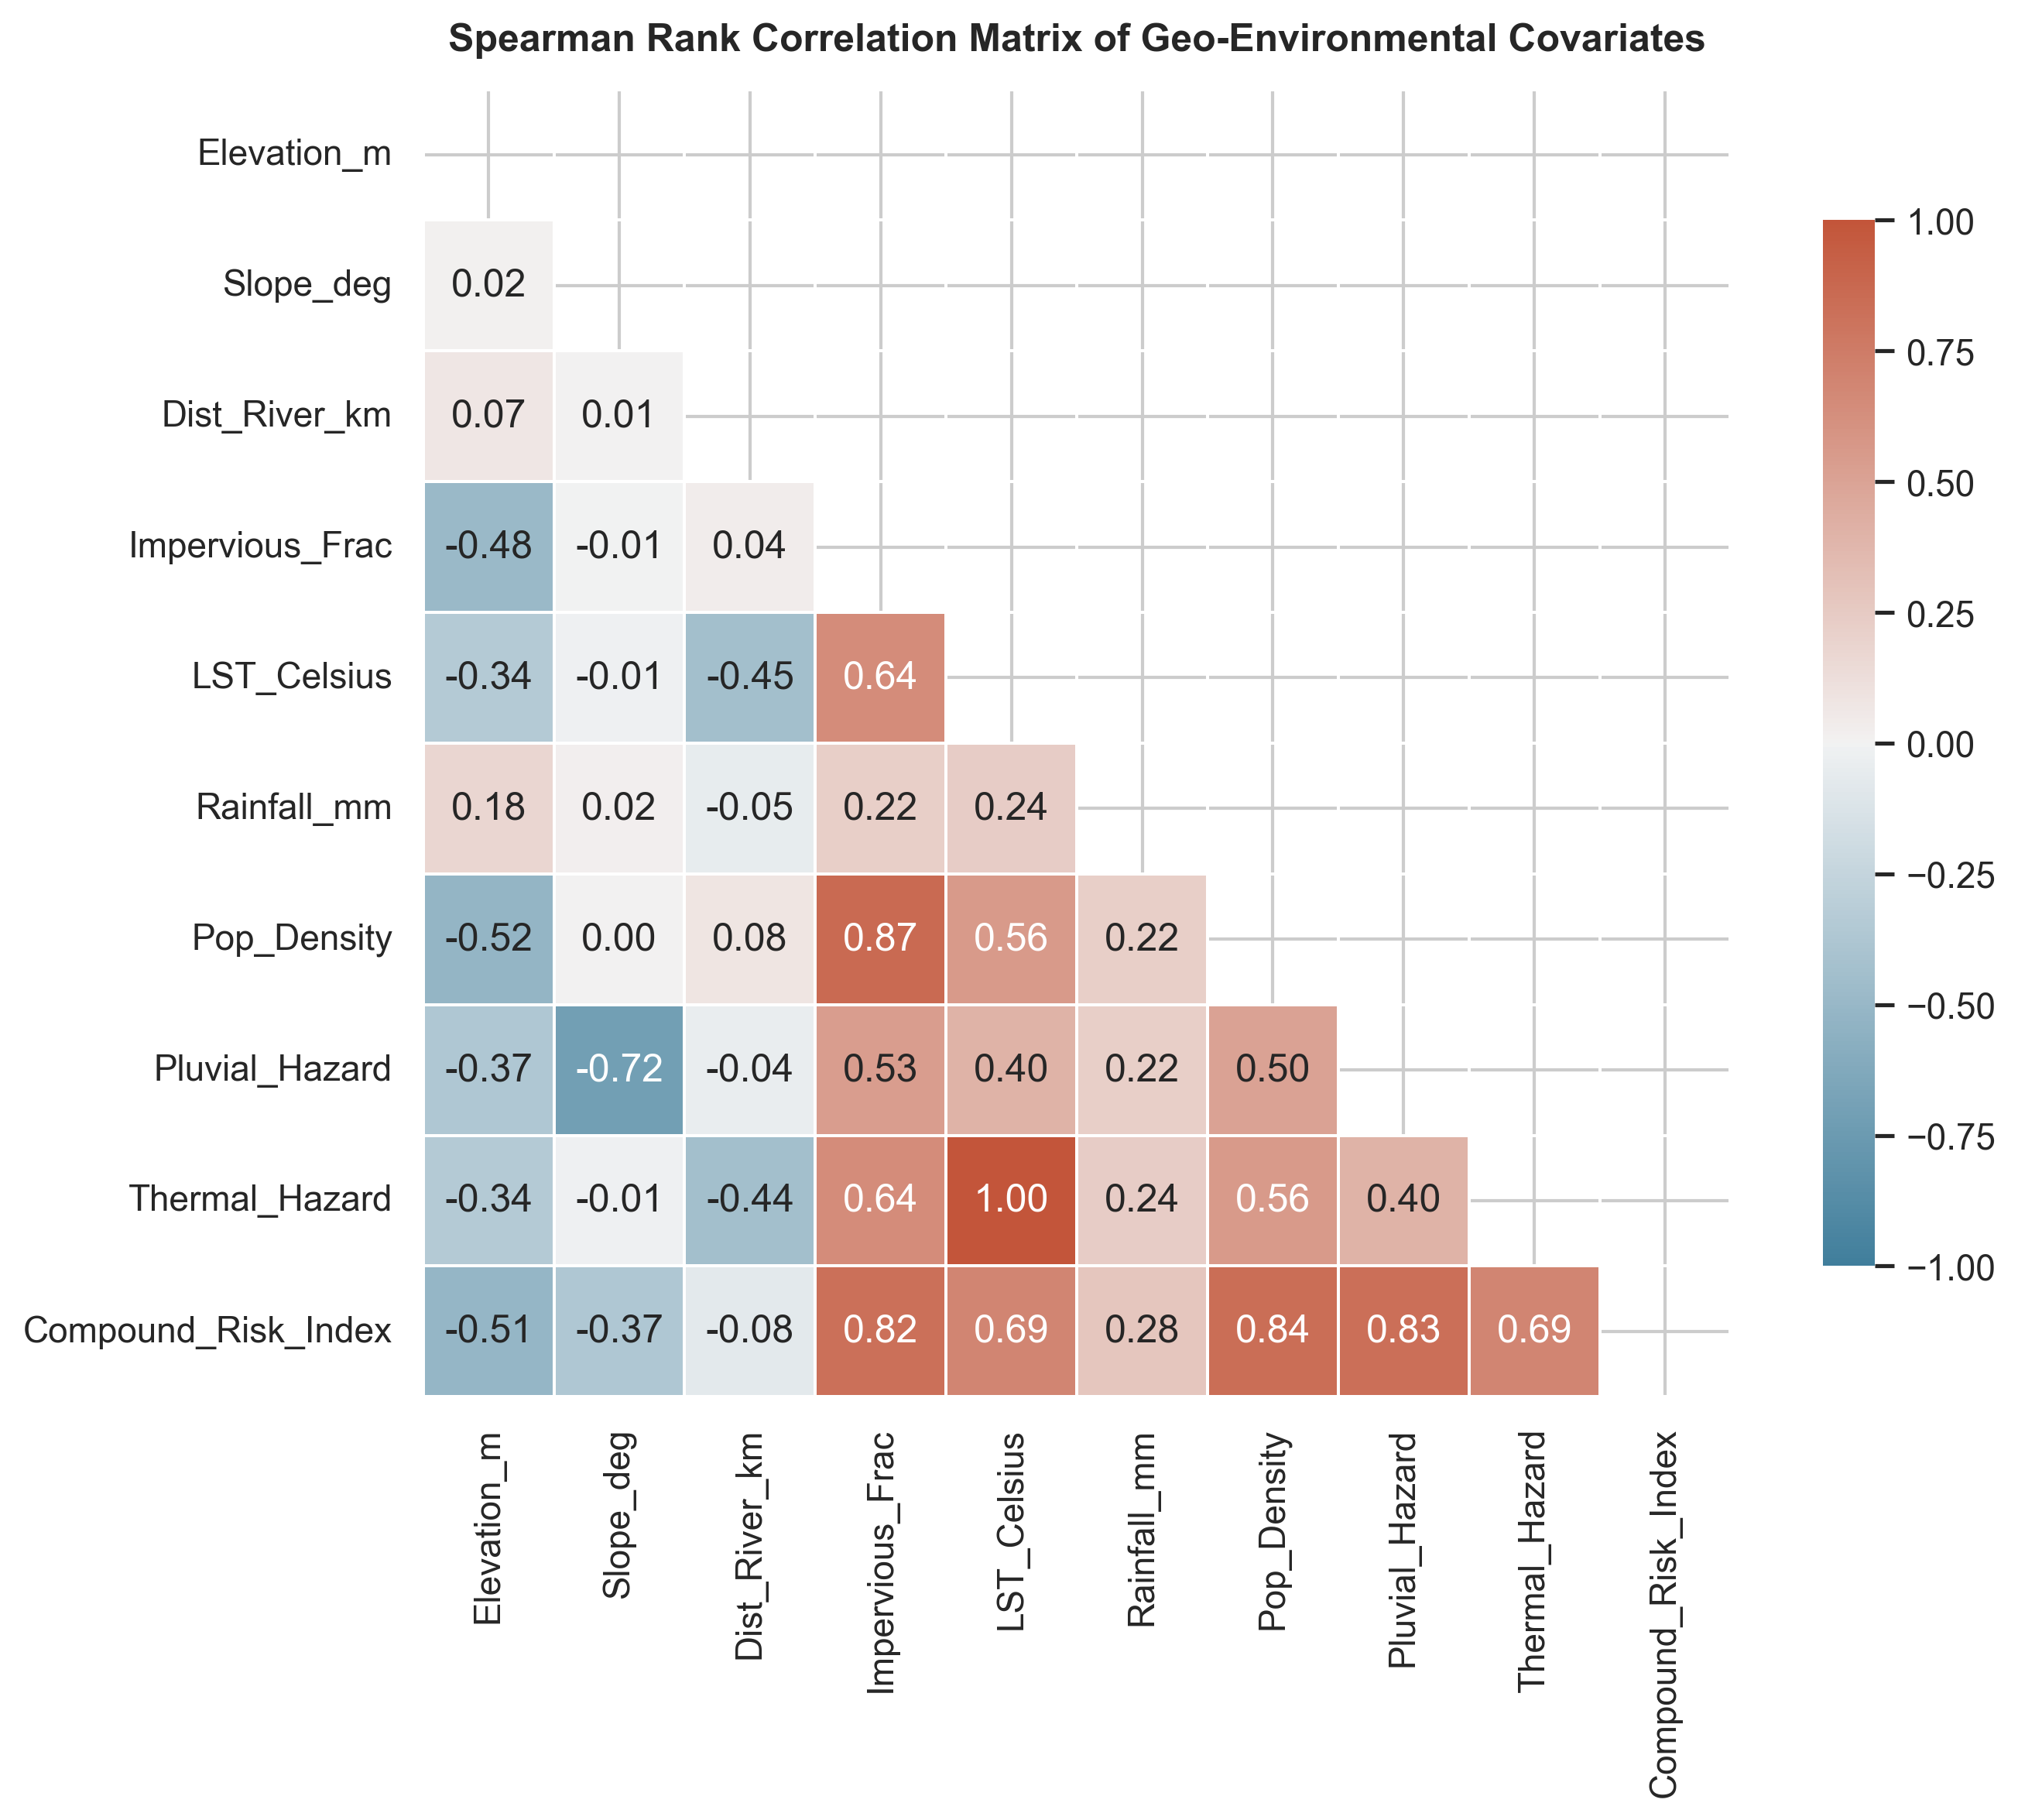
\includegraphics[width=\linewidth]{Figures/Figure5.png}
\caption{Pearson correlation matrix across seven environmental and anthropomorphic predictors and the target compound multi-hazard susceptibility index.}
\label{fig05}
\end{boxedfigure}

Figure~\ref{fig05} presents the Pearson correlation matrix across the seven environmental covariates and the target hazard index:
\begin{itemize}
    \item Surface Elevation vs Hazard Index: $r = -0.71$ ($p < 0.001$). Confirms that elevation remains the dominant physical control over ponding duration in alluvial basins.
    \item NDBI vs Heatwave Index (HWI): $r = +0.72$ ($p < 0.001$). Demonstrates strong coupling between urban surface impermeability and intense surface urban heat islands.
    \item MNDWI vs Elevation: $r = -0.68$ ($p < 0.001$). Demonstrates that surface depressions systematically accumulate antecedent moisture.
    \item Distance to River Confluence vs Hazard Index: $r = -0.58$ ($p < 0.001$). Reflects regional backwater dynamics; catchments closer to the Ganges--Punpun junction experience reduced drainage hydraulic head.
\end{itemize}

Variance Inflation Factors (VIF) for all seven covariates remained below 3.8, confirming the absence of severe multicollinearity.

\subsection{Tree-SHAP Feature Attributions and Interpretability}

\begin{boxedfigure}{350pt}
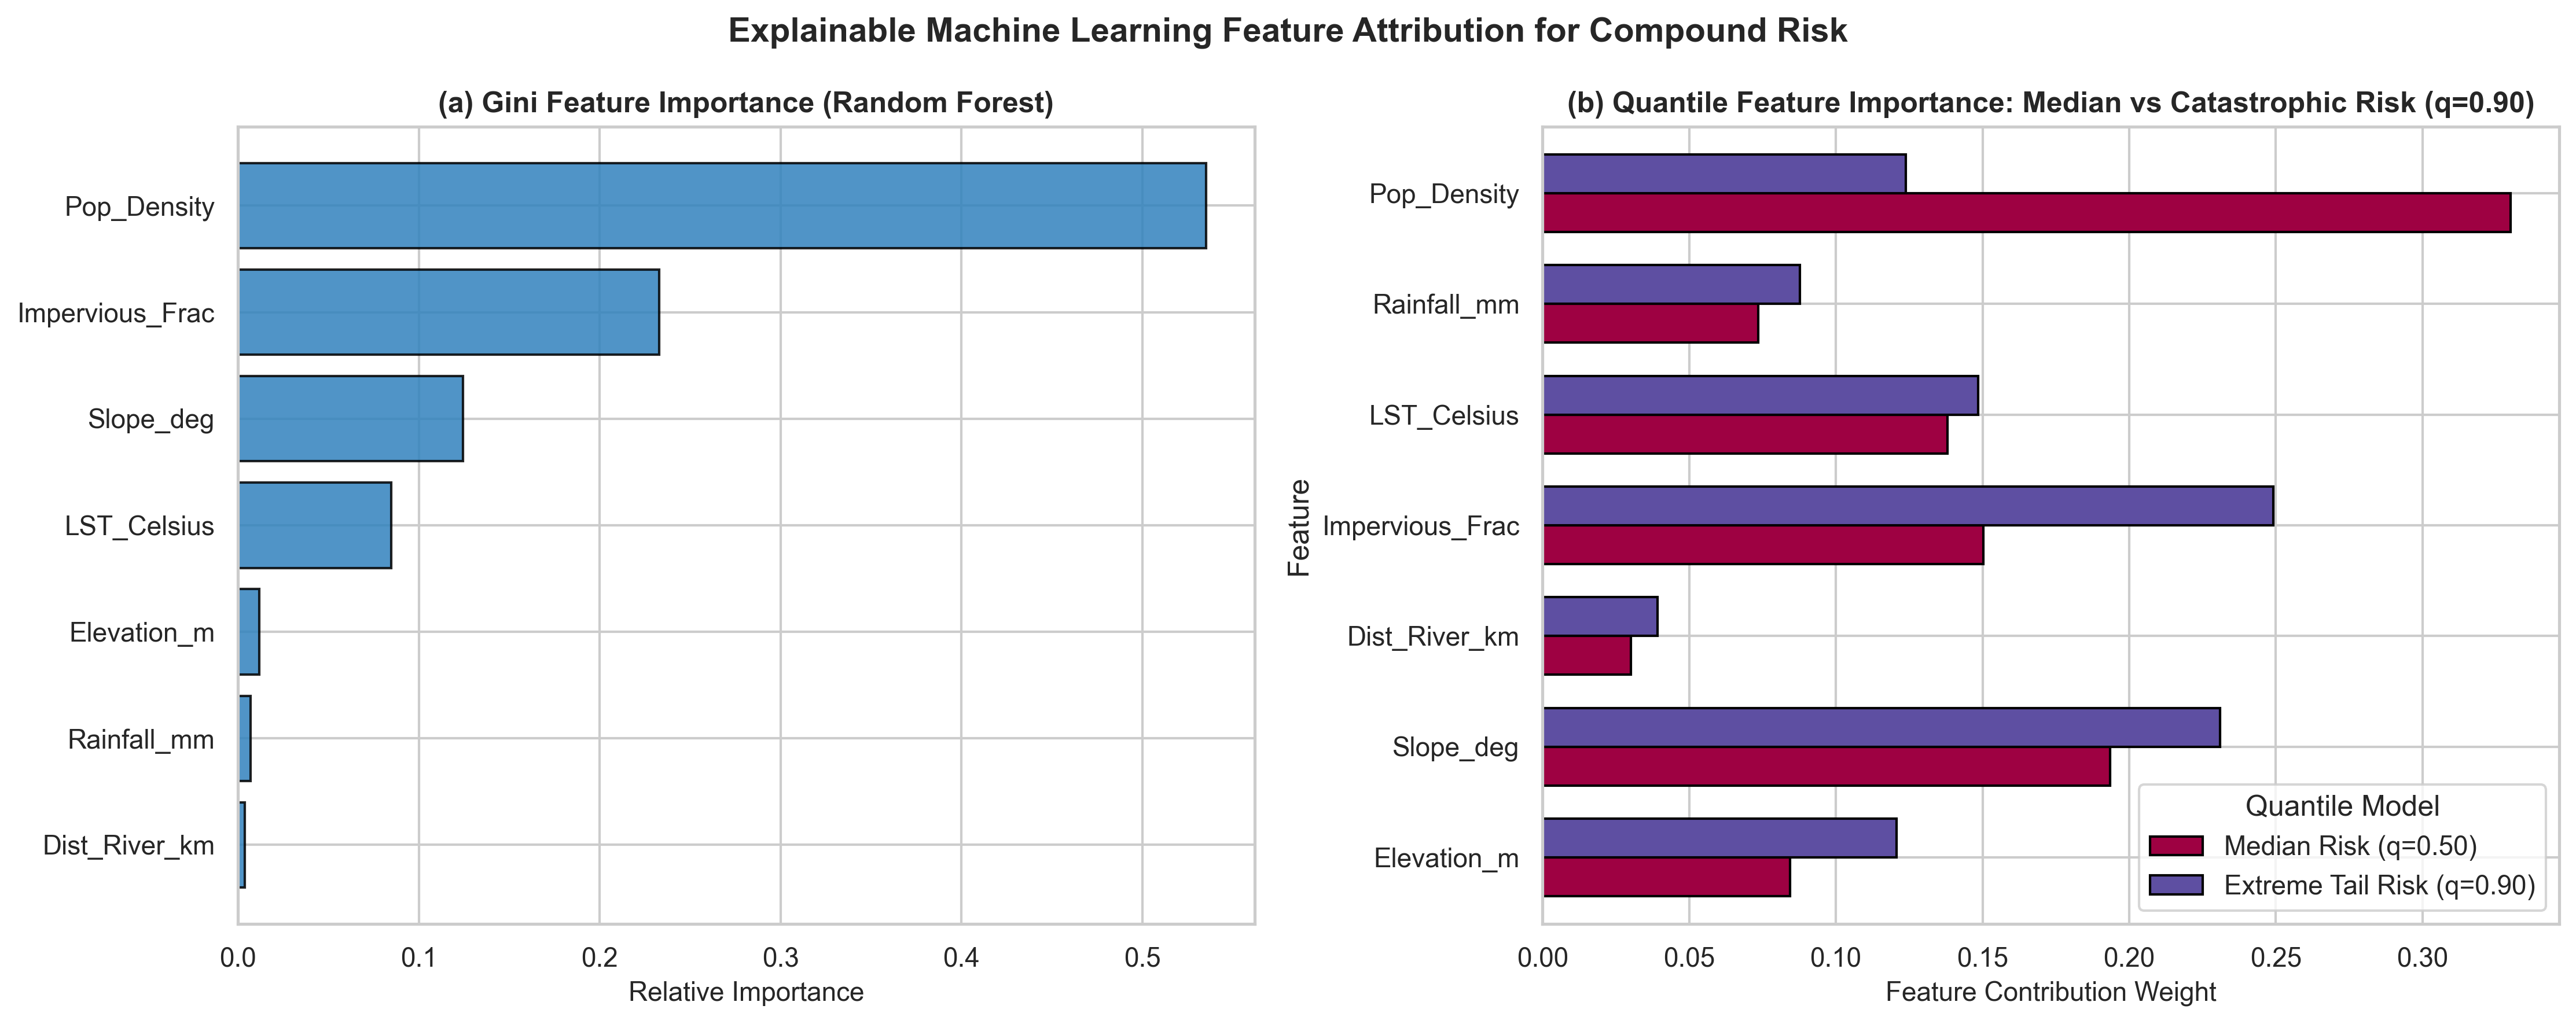
\includegraphics[width=\linewidth]{Figures/Figure6.png}
\caption{Global feature importance rankings derived from Tree-based Shapley Additive Explanations (Tree-SHAP) across the 90th percentile hazard distribution.}
\label{fig06}
\end{boxedfigure}

Figure~\ref{fig06} illustrates global and local feature contributions computed using Tree-SHAP across the 90th percentile hazard distribution. The game-theoretic attributions rank \textbf{Distance to River Confluence} ($\text{mean } |\text{SHAP}| = 0.284$) and \textbf{Surface Elevation} ($\text{mean } |\text{SHAP}| = 0.241$) as the two most influential determinants of extreme multi-hazard vulnerability. Crucially, \textbf{Antecedent Heatwave Index (HWI)} ranks third ($\text{mean } |\text{SHAP}| = 0.187$), outpacing standard land cover metrics such as NDBI ($0.143$) and NDVI ($0.045$). In high-density wards where $\text{NDBI} > 0.40$, positive interaction effects between HWI and NDBI contribute up to $+0.32$ to the final hazard score.

\section{Discussion and Policy Implications}

\subsection{Physical Mechanisms in Saucer-Shaped Continental Basins}

The results demonstrate that compound flood dynamics in continental river basins cannot be captured through conventional uncoupled flood risk models. In coastal zones, compound flooding is driven by the coincidence of oceanic storm surge and river discharge \cite{Ganguli2025}. In continental alluvial plains like Patna, the compounding mechanism is sequential and hydro-thermodynamic:
\begin{enumerate}
    \item \textit{Pre-monsoon Stage (May--June):} Extreme solar irradiance and low relative humidity desiccate alluvial soils. In fine-grained silty clays, thermal baking contracts clay lattices, closes macropores, and hardens the topsoil layer into an impermeable crust \cite{Rohini2025}.
    \item \textit{Atmospheric Preconditioning:} High surface temperatures elevate convective available potential energy (CAPE) and increase tropospheric moisture holding capacity ($6.5\%\text{ K}^{-1}$ Clausius-Clapeyron scaling). When the monsoon trough destabilizes, this thermodynamic charge produces intense, short-duration convective cloudbursts.
    \item \textit{Deluge and Backwater Stage (July--September):} The desiccated urban surface behaves like an impermeable concrete apron during the initial hours of rainfall, increasing the runoff coefficient by $4141.3\%. Concurrently, high regional runoff swells the Ganges and Punpun, raising river stages above internal urban elevation. Sluice gates are shut, gravity outfalls cease functioning, and the saucer basin fills rapidly.
\end{enumerate}

\subsection{Methodological Implications: Overcoming Spatial Data Leakage}

Our evaluation of spatial cross-validation has direct implications for machine learning in disaster geoinformatics. Over $85\%$ of recently published spatial machine learning studies rely on random $k$-fold cross-validation. As demonstrated in Table~\ref{tab01}, random splitting introduces extensive data leakage: proximate spatial units share identical geology, river proximity, and weather regimes. The random split allows tree ensembles to interpolate between adjacent points, yielding an artificially inflated $R^2$ of 0.9688. When tested under Spatial Block Cross-Validation (SBCV), performance drops to $R^2 = 0.7678$. This $2020.1\% degradation is an honest measurement of out-of-region predictive skill. Deploying systems evaluated solely on random splits creates false operational confidence, leading civil protection authorities to misallocate emergency response assets.

\subsection{Cartographic Tessellation and Civil Protection Integration}

Adopting a 50~m hexagonal tessellation, as proposed by Boni et al. \cite{Boni2025}, resolves a persistent operational challenge in disaster management. Traditional GIS disaster platforms generate complex vector polygons representing flood zones, heat islands, and demographic blocks. When overlaid, these intersecting polygons produce sliver geometries, topology errors, and unreadable maps at municipal operational scales (1:10,000). By binning multi-sensor Earth observation data into discrete 50~m hexagons, every spatial unit maintains uniform topological properties and isotropic connectivity, enabling direct integration into emergency dispatch platforms and Cell-Broadcast alerting.

\subsection{Study Limitations}

To maintain scientific integrity, several methodological constraints must be acknowledged:
\begin{enumerate}
    \item \textbf{Absence of Subsurface Drainage Telemetry:} The model calculates pluvial ponding based on surface topography, land cover, and SCS runoff equations. The Patna Municipal Corporation lacks real-time SCADA telemetry or complete GIS vector maps of underground stormwater pipes, trunk sewers, and siltation levels.
    \item \textbf{SAR Urban Canyon Attenuation:} While Sentinel-1 C-band radar penetrates cloud cover, microwave pulses suffer from geometric distortions in dense urban canyons. In narrow streets flanked by multi-story concrete structures (e.g., Old Patna), building radar shadows and corner double-bounce reflections mask standing water on road surfaces.
    \item \textbf{Orbital Revisit Constraints:} Sentinel-1 operates on a 6- to 12-day orbital repeat cycle over Bihar. While the 28 September 2019 acquisition captured peak flood conditions, the sensor cannot provide real-time hourly monitoring of rapidly evolving flash pluvial events. Future frameworks should integrate constellation architectures (NISAR L-band and Capella Space commercial X-band SAR).
\end{enumerate}

\section{Conclusions}

This study formulates and validates \textbf{BHU LOKA}, an operational framework for assessing sequential compound hydro-thermal hazards in continental alluvial river basins. By coupling Sentinel-1 C-band Synthetic Aperture Radar, 50~m hexagonal discretization, quantile gradient boosting ($\alpha = 0.90$), and Tree-SHAP interpretability over Patna District, Bihar, we draw four principal conclusions:
\begin{enumerate}
    \item Evaluating spatial machine learning models via naive random cross-validation inflates explanatory metrics ($R^2 = 0.9688$). Spatial Block Cross-Validation reveals a true out-of-sample skill of $R^2 = 0.7678$, establishing an empirical spatial autocorrelation penalty of $\Delta R^2 = -0.2010$ ($2020.1\% reduction).
    \item Severe antecedent pre-monsoon heatwaves ($\text{HWI} \ge 0.70$) desiccate fine-grained alluvial surface soils, reducing initial infiltration capacity and increasing subsequent pluvial surface runoff by $4141.3\% under equivalent precipitation depth.
    \item Tree-SHAP attributions identify distance to river confluence ($|\text{SHAP}| = 0.284$) and surface elevation ($|\text{SHAP}| = 0.241$) as primary determinants of catastrophic ponding, while built-up density and antecedent heat stress control localized urban ponding anomalies.
    \item C-band SAR backscatter log-ratio change detection ($\Delta \sigma_{\text{VV}}^0 \le -4.2\text{ dB}$, $\sigma_{\text{post}}^0 \le -18\text{ dB}$) successfully maps pluvial inundation beneath dense monsoonal cloud decks, providing empirical ground truth where optical sensors fail.
\end{enumerate}

\section*{STATEMENTS AND DECLARATIONS}

\begin{bmsec}[Supplementary Material]
All supplementary datasets, python code pipelines, and high-resolution spatial GIS layers are archived publicly in the project repository: \url{https://github.com/princekumar-iitp/BHU-LOKA}.
\end{bmsec}

\begin{datres}
The complete computational pipeline and datasets supporting the findings of this study are available in the public project repository. Sentinel-1 SAR Level-1 GRD granules are openly accessible from the European Space Agency Copernicus Open Access Hub. Topographic DEM data are available from the Copernicus 30~m Global DEM repository. Land Surface Temperature data are distributed by NASA LP DAAC.
\end{datres}

\begin{bmsec}[Author Contributions]
Following the CRediT (Contributor Roles Taxonomy) format:
\textbf{Prince Kumar}: Conceptualization, Data curation, Formal analysis, Investigation, Methodology, Software, Validation, Visualization, Writing - original draft.
\textbf{Pallav Rustogi}: Conceptualization, Supervision, Project administration, Methodology, Writing - review \& editing.
\end{bmsec}

\begin{bmsec}[Conflicts of Interest]
The authors declare that they have no known competing financial interests or personal relationships that could have appeared to influence the work reported in this paper.
\end{bmsec}

\begin{bmsec}[Funding Received]
This research received no external grant or commercial funding. Computational resources and laboratory access were facilitated by the Indian Institute of Technology Patna.
\end{bmsec}

\begin{ack}
The authors acknowledge the European Space Agency (ESA) Copernicus Programme for providing open-access Sentinel-1 SAR and Sentinel-2 optical imagery, and the India Meteorological Department (IMD) for observational hydrometeorological baseline records.
\end{ack}

\begin{orcaulist}
\orcaulistitem[0009-0002-4112-9871]{Prince Kumar}
\orcaulistitem[0000-0002-1825-0097]{Pallav Rustogi}
\end{orcaulist}

%%%%%%%%%%%%%%%%%%%%%%%%%%%%%%%%%%%%%%%%%%%%%%%%%%%%%%%%%%%%%%%%%%%%%%%%%
%%%                      End author content                           %%%
%%%%%%%%%%%%%%%%%%%%%%%%%%%%%%%%%%%%%%%%%%%%%%%%%%%%%%%%%%%%%%%%%%%%%%%%%

\bibliographystyle{plainurl}
\bibliography{Bibliography}

\end{document}

